\documentclass[tikz]{standalone}

\usepackage[latin1]{inputenc}
\usepackage{tikz}
\usetikzlibrary{patterns}
% GNUPL
\begin{document}
\pagestyle{empty}


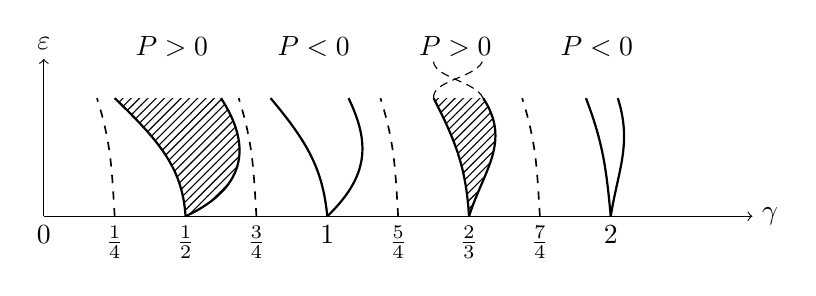
\begin{tikzpicture}[scale=0.5, xscale=1.8]
    %\draw[very thin,color=gray] (-1,1.1) grid (3.9,3.9);
    \draw[->] (0,0) -- (10,0) node[right] {$\gamma$};
    \draw[->] (0,0) -- (0,4) node[above] {$\varepsilon$};
    
    \draw [black, dashed, semithick] (1,0) to [out=92,in=-80] (0.75,3);
    \draw [black, dashed, semithick] (3,0) to [out=92,in=-80] (2.75,3);
    \draw [black, dashed, semithick] (5,0) to [out=92,in=-80] (4.75,3);
    \draw [black, dashed, semithick] (7,0) to [out=92,in=-80] (6.75,3);
 
    \draw [draw=none,pattern=north east lines,opacity=1] (2,0) to [out=92,in=-60] (1,3) -- (2.5,3) to [in=40,out=-70] (2,0);
    \draw [black, thick] (2,0) to [out=92,in=-60] (1,3);
    \draw [black, thick] (2,0) to [out=40,in=-70] (2.5,3);
    
    \draw [black, thick] (4,0) to [out=93,in=-65] (3.2,3);
    \draw [black, thick] (4,0) to [out=60,in=-75] (4.3,3);


    \draw [draw=none,pattern=north east lines,opacity=1] (6,0) to [out=92,in=-74] (5.5,3) -- (6.2,3) to [in=80,out=-70] (6,0);

    \draw [black, thick] (6,0) to [out=92,in=-74] (5.5,3);
    \draw [black, thick] (6,0) to [out=80,in=-70] (6.2,3);

    \draw [black, densely dashed] (5.5,3) to [out=93,in=-95] (6.2,4);
    \draw [black, densely dashed] (6.2,3) to [out=105,in=-95] (5.5,4);

    \draw [black, thick] (8,0) to [out=93,in=-78] (7.65,3);
    \draw [black, thick] (8,0) to [out=85,in=-80] (8.1,3);


    \draw (2,3.8) node[above, xshift=-5pt] {$P>0$};   
    \draw (4,3.8) node[above, xshift=-5pt] {$P<0$};   
    \draw (6,3.8) node[above, xshift=-5pt] {$P>0$};   
    \draw (8,3.8) node[above, xshift=-5pt] {$P<0$};   

    \coordinate [label=-90:$0$] (0) at (0,0);
    \coordinate [label=-90:$\frac14$] (1) at (1,0);
    \coordinate [label=-90:$\frac12$] (sdfdf) at (2,0);
    \coordinate [label=-90:$\frac23$] (sdfdf) at (6,0);
    \coordinate [label=-90:$\frac34$] (2) at (3,0);
    \coordinate [label=-90:$1$] (3) at (4,0);
    \coordinate [label=-90:$\frac54$] (4) at (5,0);
    \coordinate [label=-90:$\frac74$] (5) at (7,0);
    \coordinate [label=-90:$2$] (6) at (8,0);
    % \coordinate [label=-90:$P<0$] (7) at (1.8,2);
    % \coordinate [label=-90:$P<0$] (7) at (5.8,2);
    % \coordinate [label=-90:$P>0$] (7) at (3.8,2);
    % \coordinate [label=-90:$P>0$] (7) at (7.8,2);
    % \draw [black, thick] [->] (2,3.5)--(1,3.2);
    % \draw [black, thick] [->] (2.7,3.5)--(2.7,3.2);
    % \draw [black, thick] [->] (3.2,3.7)--(4.6,3.2);
    % \coordinate [label=-90:$P\equiv0$] (8) at (2.6,4);

    % \draw [green, thick] (1.93,0.7) -- (2.55,0.7);
    % \draw [green, thick] (1.81,1.3) -- (2.72,1.3);
    % \draw [green, thick] (1.58,1.9) -- (2.75,1.9);
    % \draw [green, thick] (1.28,2.5) -- (2.65,2.5);
    % \draw [red, thick] (3.9,1)--(4.58,1);
    % \draw [red, thick] (3.63,2)--(4.55,2);
    % \draw [green, thick] (5.93,1) -- (6.48,1);
    % \draw [green, thick] (5.96,0.5) -- (6.33,0.5);
    % \draw [green, thick] (5.86,1.5) -- (6.53,1.5);
    % \draw [green, thick] (5.76,2) -- (6.48,2);
    % \draw [red, thick] (7.93,1)--(8.38,1);
    % \draw [red, thick] (7.84,2)--(8.31,2);
\end{tikzpicture}


\end{document}